\chapter{绪论}
\label{chap:introduction}

本章的内容包括实体关系知识抽取的研究背景与其意义,阐释了在当先信息大爆炸的时代里,如何从不计其数的信息中提取出实体,之后从实体之间抽取出关系元组来建立全面而准确的信息知识数据库,从而更好地服务互联网的使用者。也介绍了国内外对于本课题的研究现状和本文的研究内容,以及概述中文开放式关系抽取系统中所使用的机器学习算法。

\section{研究背景与意义}

\subsection{研究背景}

传统的信息提取涉及很多人为因素的干扰,包括以手工制定的规则或手工标注出来的样例来作为机器学习的预定义参数,之后才能识别并判断在输入的文本中两个实体之间的特定关系\citep{wang}。即使机器学习可以帮助枚举出潜在的可供提取的关系模式,但这个方式常常只能提取已经被预定义的关系集。并且,这个方式不适用于如今的互联网,因为其当中的信息大都是非结构化、未预先定义实体关系的。

另一种开放的信息抽取\citep{banko}方式则不需要人工对每种关系类型进行预定义,它可以从文本抽取关系并能方便地度量网络语料库的多样性和覆盖范围。语料库是开放式信息抽取系统所需要的唯一一种输入数据,它的输出则是被抽取出的各种关系的集合。一个开放式信息抽取系统通过它的语料库大小来控制它所能抽取关系的可扩展性,并用以下方法来增加可处理的关系类型:基于浅分析、基于语法或没有预定义关系的基于词法分析的模式匹配\citep{wu2010, naka2012, etz2011}。现在的开放式关系抽取技术关注于字面上关系的抽取,而没有尝试进行词法分析,但词法分析却是传统信息抽取的优点。

\subsection{研究意义}
中文开放式关系抽取外的其他的开放式关系抽取系统是抽取二元的关系,之后将其归纳为语义模式。而中文开放式关系抽取则同时进行抽取关系和归纳模式,利用双重拓展的算法让关系和模式信息互相加固加强,从而减弱自动词法分析和自动语义分析所带来的负面影响,语义模式信息可以帮助提升关系抽取的质量。所以本次毕设采用了中文开放式关系抽取做为关系抽取的引擎。

\section{开放式关系抽取的基本定义}
中文开放式关系抽取被应用于网络文本来提取普遍意义上的关系和它们的语义类型。对于关系的定义大部分都是来自于英文语境下,但是此次毕设的语义环境处在中文里,所以需要对基于英文语境下的开放式关系抽取进行一些适合中文语境的调整。以下的概念定义以句子“侯建国校长就职于中国科学技术大学。”做为样例。

\begin{figure}[ht]
\centering
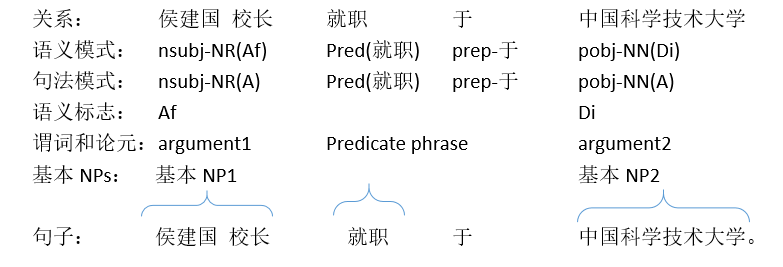
\includegraphics[width=15cm]{sentence1}
\caption{分析样例句子}\label{fig:sentence1}
\end{figure}

\subsection{谓词短语(predicate phrase)}
谓词短语是包括至少一个动词或系词,并在语句构成上控制至少一个名词的词语序列。例如,图 ~\ref{fig:sentence1} 里的谓词短语是“就职”。为了预防“少动词结构”的情况出现,动词和它所直接“控制”的对象共同被认为是一个“谓词短语”。介词并不被包括在谓词短语的范围中。

\subsection{论元(argument)}
论元是一个被谓词短语所直接控制或通过介词间接控制的基本名词短语。例如,图 ~\ref{fig:sentence1} 里的“侯建国校长”和“中国科学技术大学”就是谓词短语“就职”的两个论元。

\subsection{关系(relation)}
一个“二元关系”是一个包括了谓词短语 pred 和它的两个论元 x 与 y 的三元组。依此类推,一个“n 元关系”则包括了 n 个论元。例如,图 ~\ref{fig:sentence1} 里的句子包含了一个二元关系(x[侯建国校长], pred[就职], y[中国科学技术大学])。在英文语境下,二元关系的两个论元通常分别位于 pred 的左边和右边。因此,弱模式对于英文语境下的的关系抽取非常有效。然而在中文语境下,二元关系的两个关系有可能都在 pred 的左边(例如“我和你打架”),都在 pred 的右边(例如“抄袭了我的作业”),或者一左一右分布在 pred 的两边,即根据不同的句子,出现的关系模式可能为(x, y, pred),(pred, x, y)和(x, pred, y)。从而让关系短语的探测变得更加复杂。

\subsection{句法模式(syntactic pattern)}
句法模式是一个关系的句法抽象,一个关系可以被推广到字词的组合、POS 标签(Part of speech,词性标注标签)和句法依赖标志。例如,图 ~\ref{fig:sentence1} 中的句法模式是\{nsubj-NR(A), Pred[就职], prep-于, pobj-NN(A)\}。它由四个子模式组成。第一个子模式 nsubj-NR(A) 表示当前的短语扮演着具有 POS 标签 NR (proper nouns,专有名词)的谓词短语的主语,在这里(A)意味着这个短语是被提取出的关系中的论元。第二个子模式表示图 ~\ref{fig:sentence1} 中的样例句子谓词短语是“就职”。并且在谓词和论元中的字词(例如 prep-于)被直接包括在模式中。

\subsection{语义标志(semantic signature)}
一个关系里的语义标志包括着论元的语义分类。图 ~\ref{fig:sentence1} 中的语义标志是(Af, Di),其中 Af 表示“人类”,Di 表示“院校”。

\subsection{语义模式(semantic pattern)}
语义模式是一个关系里的语义抽象。它是由句法模式和语义标志结合成的。例如,句法模式\{nsubj-NR(A), Pred[就职], prep-于, pobj-NN(A)\}与语义标志(Af,Di)结合,就生成了语义模式{nsubj-NR(Af), Pred[就职], prep-于, pobj-NN(Di)}。

\section{机器学习相关算法}
\subsection{聚类}
\subsubsection{基本概念}
聚类即将实体根据他们之间具有的属性进行处理,有相似属性的则聚集为一个类别,使得聚集出的同一种类别内部的所有实体之间都具有较高的相似性,而不是属于同一种类别的实体之间的相似性则较低。对聚类算法的度量主要是度量其使用的计算相似性和距离的方法。

对实体进行聚类,需要对不同实体之间的相似度和距离进行计算。即两个实体之间的距离越近,则他们的相似度就越高,也就是由更高的可能性被归类到同一个类别中。常见的距离和相似度计算度量类别较多,将结合公式在下文进行介绍,以两个 m 维向量 $X = (x_1, x_2 ......, x_m)$ 和 $Y = (y_1, y_2 ......, y_m)$ 表示两个实体之间的相似度和距离计算公式, $S_{ij}$ 和 $D_{ij}$ 分别代表两个向量之间的相似度和距离。
\newtheorem*{oujilide}{欧几里得距离}
\begin{oujilide}
    \begin{equation}
        d_{ij}(X,Y) = \sqrt{\sum_{k=1}^m|{x_k - y_k}|^2}
    \end{equation}
\end{oujilide}

\newtheorem*{yuxian}{余弦相似度}
\begin{yuxian}
    \begin{equation}
        S_{ij}(X, Y) = cos(\theta) = \frac{\sum_{k=1}^mx_ky_k}{\sqrt{\sum_{k=1}^mx_k^2}\sqrt{\sum_{k=1}^my_k^2}}
    \end{equation}
\end{yuxian}

\newtheorem*{manhadun}{曼哈顿距离}
\begin{manhadun}
    \begin{equation}
        d_{ij}(X,Y) = \sum_{k=1}^m|x_k-y_k|
    \end{equation}
\end{manhadun}

\newtheorem*{qiebixuefu}{切比雪夫距离}
\begin{qiebixuefu}
    \begin{equation}
        d_{ij}(X,Y) = \max \limits_{1 \leq k \leq m}|x_k - y_k|
    \end{equation}
\end{qiebixuefu}

\newtheorem*{xiangguanxishu}{相关系数}
\begin{xiangguanxishu}
    \begin{equation}
        d_{ij}(X,Y) = \frac{\sum_{k=1}^m(x_k-\overline{X})(y_k-\overline{Y})}{\sqrt{\sum_{k=1}^m(x_k-\overline{X})}\sqrt{\sum_{k=1}^m(y_k-\overline{Y})}}
    \end{equation}
\end{xiangguanxishu}

\newtheorem*{mingkefusiji}{名科夫斯基距离}
\begin{mingkefusiji}
    \begin{equation}
        d_{ij}(X,Y) = \left( \sum_{k=1}^m|x_k-y_k|^q \right) ^ \frac{1}{q}, q > 0
    \end{equation}
\end{mingkefusiji}

若名氏距离里的 $q=0$ 则为曼哈顿距离,$q=1$ 则为欧几里得距离,$q\to \infty$ 则为切比雪夫距离。

\subsubsection{几种不同的聚类方法}
因为互联网数据的类别和数量都很多,所以目前没有一个普适的聚类算法可以用来对每种类型的数据进行梳理。需要使用算法处理特定类型的数据时,应该考虑待处理数据的特点、聚类的目的及使用场景。如图 ~\ref{fig:cluster}。

\begin{figure}[ht]
\centering
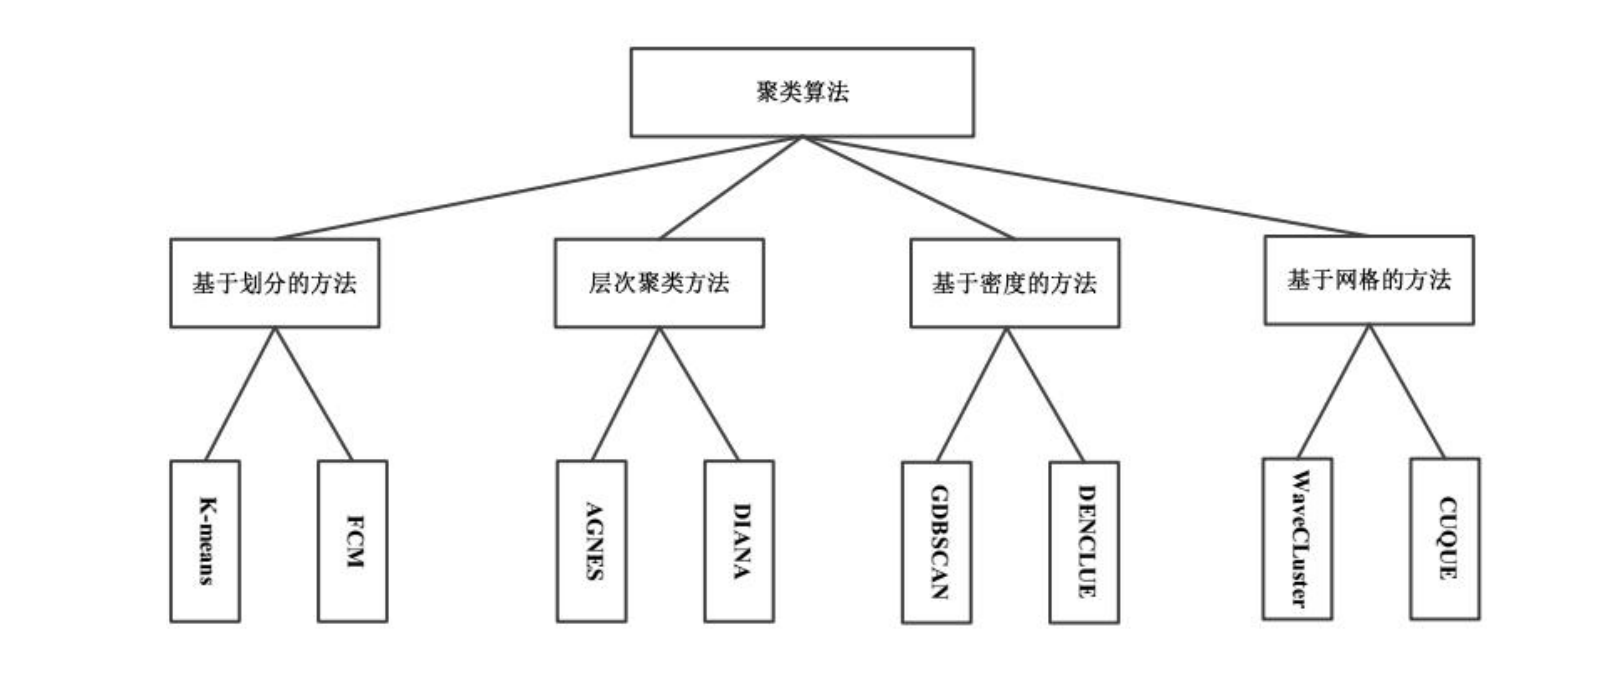
\includegraphics[width=13cm]{cluster}
\caption{聚类算法的归类}\label{fig:cluster}
\end{figure}

\newtheorem*{huafenfa}{基于划分的方法}
\begin{huafenfa}
    该方法为把有 n 个元素的数据集分割成 k 个子集,$k \leq n$。而划分结果中的每一个子集就是一个类别,也就是聚类之后的一个簇。而 K-means 算法,即是最经典的基于划分的聚类方法。
\end{huafenfa}

\newtheorem*{cengcijuleifa}{层次聚类方法}
\begin{cengcijuleifa}
    这个方法是将数据集以逐层进行的方法来处理,方向有自下而上,也有自上而下。而两个方向则分别是合并小类别(凝聚层级聚类)与将大类别分割(分裂层次聚类)。凝聚层次聚类就是对每种小类别进行迭代地合并直至达到结束条件,而算法初始时,将数据集的每个元素都视为一个类别,该聚类方法的典型算法是 $AGNES$ 算法。分裂层次聚类则与凝聚层次聚类相反,是对每种类别进行迭代地分割,直至达到算法结束条件,算法初始下,将整个数据集视为一个类别,这种方法的典型算法则为 $DIANA$ 算法。
\end{cengcijuleifa}

\newtheorem*{midufa}{基于密度的方法}
\begin{midufa}
    该方法为依据所给的数据元素的密度,将其划分为不同的类别。即把数据元素组成的每个类别看成是散布在空间中的各自独立的区域。若数据集当中的邻接点达到了定下的阈值则停止聚类,否则继续进行,直至生成大量的类别。$GDBSCAN$,$DENCLUE$ 都是密度聚类的经典算法。
\end{midufa}

\newtheorem*{wanggefa}{基于网格的方法}
\begin{wanggefa}
    该方法为通过网格技术把所给的数据集分割为互相独立的网格结构,对在网格内部的数据采取聚类操作。这种方法的优势为聚类的时间复杂度与数据集内部的元素数无关,而是与网格数有关。而其性能则由划分的网格结构底层粒度决定,若粒度变细,则处理代价变大。对上层的单元分割时,统计信息网格并未将底层与其邻元的关系纳入考虑,所以这种方法时间复杂度虽然较低,但其生成的聚类结果精确性可能不尽如人意。$WaveCluster$,$CUQUE$ 都是经典的网格聚类算法。
\end{wanggefa}

\subsubsection{K-means 算法}
由之前的介绍我们已经知道,K-means 是一种经典的划分聚类算法,由数据之间的距离来度量其相似性,即距离越近,相似性越大。

算法 ~\ref{algo:kmeans} 的详细工作步骤为,第一步,随机生成 k 个点的坐标作为 k 个类别的起始中心坐标;第二步,对数据集内的每个元素都计算其与制定类别的起始中心距离,把当中样本的数据纳入离它最近的起始中心的类别的类,即得出了了起始的 k 个类别分布;第三步,接着对经过第二步处理的数据重新计算他们所属类别的中心坐标,之后执行与第二步相同的过程,若类别中心与之前的类别中心相同则算法结束,不然就接着重复第三步的过程,最后会得出收敛的 k 个类别的中心坐标。

\begin{algorithm}[!h]
\SetAlgoLined
\KwData{$n$ 个数据对象 $x_i$ 的集合 $X$}
\KwResult{$k$ 个聚类中心 $C_j$ 以及 $k$ 个类别的数据集合 $D_j$}
\SetKw{KwIns}{insert}
\SetKw{KwInt}{into}
\SetKw{KwT}{true}
\SetKw{KwF}{false}
    $flag = $\KwT \;
    initial $k$ protottype $C_j, j \in \left[ 1, k \right]$ \;
    \While{$flag$}{
        \For{$i \leftarrow 1$ \KwTo $n$}{
            $D\left( x_i, c_j \right) \leftarrow |x_i - c_j|$\;
        }
        \uIf{$D\left( x_i, c_j \right) = \min \{ D\left( x_i, c_j \right) \} $}{
            \KwIns $x_i$ \KwInt $D_j$\;
        }
        \uIf{$C_j$ changed}{
            $c_j \leftarrow \frac{1}{N} \sum_{p=1}^{N_j}x_{jp}, j \in 1,2, ......, k$\;
        }
        \Else{
            $flag =$ \KwF \;
        }
    }
\caption[K-means 算法]{K-means}
\label{algo:kmeans}
\end{algorithm}

\subsection{$Logistic$ 回归}
$Logistic$ 算法为一个经典的且应用广阔的机器学习算法。大致思想为通过计算得到的样本数据所属的每种类别的概率来推测其他样本所属的类别。

设想有一个训练数据集 $X$,其元素个数为 $n$ 个, $X = \{ x_1,x_2,......,x_n\}$,每个元素对应的类型标签 $Y=\{ y_1,y_2,......,y_n\}$,每个元素 $x_i$ 的维度是 $d$,形式是 $x=\left[ x^{\left( 1\right)},x^{\left( 2\right)},......,x^{\left( n\right)} \right] ^T, y \in \{ 1,2,......,c\}$。
\newtheorem*{yucehanshu}{预测函数}
\begin{yucehanshu}
    \begin{equation}
        h_{\theta}\left( x\right) =g\left( \theta^Tx\right) =\frac{1}{1+e^{-\theta^Tx}} \in \left[ 0,1 \right]
    \end{equation}
    其中的向量 $\theta$ 是需要学习的参数。
\end{yucehanshu}

\newtheorem*{sigmoid}{$Sigmoid$函数}
\begin{sigmoid}
    \begin{equation}
        g\left( z\right) =\frac{1}{1+e^{-z}} \in \left[ 0,1 \right]
    \end{equation}
\end{sigmoid}

而为了在实际使用中的便利性,令$x^{\left( 0 \right)} =1$,即 $\theta^Tx=\sum_{j=0}^d\theta_jx^{\left( j \right)}$。

算法的学习就是利用计算过程来获取 $\theta$,定义损失函数,之后以极大似然估计或最小化损失函数对 $\theta$ 进行计算。接下去以极大似然估计法来计算 $\theta$,假设 $X, Y$ 分别为样本集和其元素的归属类别集,二者互相独立,则每个样本的联合分布可由该样本的边际分布的乘积所求出。

\newtheorem*{jidasiran}{$\theta$ 的极大似然估计函数}
\begin{jidasiran}
    \begin{equation}
        L\left( \theta \right) = \prod_{i=1}^nP\left( y_i|x_i,\theta \right) = \prod_{i=1}^nh_{\theta}\left( x_i \right)^{y_i}\left(1-h_{\theta}\left(x_i \right) \right)^{1-y_i}
    \end{equation}
\end{jidasiran}

\newtheorem*{sunshihanshu}{损失函数}
\begin{sunshihanshu}
    \begin{equation}
        J\left( \theta \right) = -\frac{1}{n}\left( \sum_{i=1}^n\sum_{k=1}^nI\{ y_i=k\} log\frac{e^{\theta_k^Tx}}{\sum_{l=1}^ce^{\theta_l^Tx}} \right)
    \end{equation}

    当中 $I\{ y_i=k\}$ 即为指示器函数,如果 $y_i=k$ ,$I\{ y_i=k\} =1$,否则 $I\{ y_i=k\} =0$。
\end{sunshihanshu}
